\documentclass[tikz,border=10pt]{standalone}
\usepackage{tkz-euclide} % 专门用于几何作图的宏包

\begin{document}
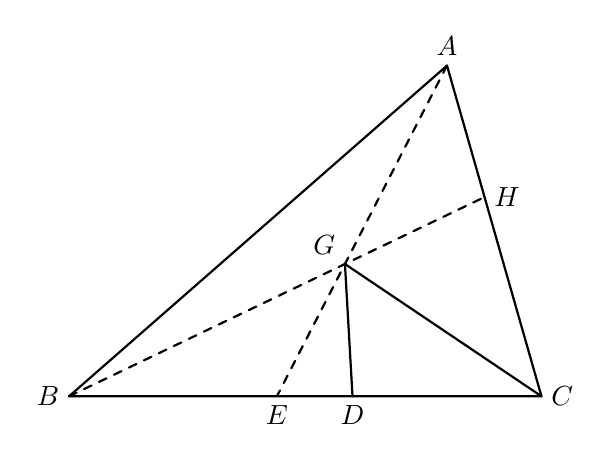
\begin{tikzpicture}[scale=1.2, line join=round, line cap=round]
    % 1. 定义顶点坐标 (根据原图比例粗略设定)
    \coordinate (B) at (0, 0);
    \coordinate (C) at (5, 0);
    \coordinate (A) at (4, 3.5);

    % 2. 计算点的位置 (依据图中视觉几何关系)
    % D 在 BC 上 (约在中点右侧)
    \coordinate (D) at (3, 0);
    % E 在 BC 上 (在 D 的左侧)
    \coordinate (E) at (2.2, 0);
    % G 是内部的一个关键交点 (通过 A 与 E 的连线以及 B 的射线确定)
    % 这里设定 G 在 AE 上
    \coordinate (G) at (barycentric cs:A=0.4,E=0.6);
    % H 在 AC 上，由 BG 的延长线与 AC 相交得到
    \coordinate (H) at (intersection of B--G and A--C);

    % 3. 绘制实线部分 (主要轮廓)
    \draw[thick] (A) -- (B) -- (C) -- cycle; % 三角形 ABC
    \draw[thick] (G) -- (D); % 线段 GD
    \draw[thick] (G) -- (C); % 线段 GC

    % 4. 绘制虚线部分 (辅助线或内部构造线)
    \draw[dashed, thick] (A) -- (E); % 线段 AE 过点 G
    \draw[dashed, thick] (B) -- (H); % 线段 BH 过点 G

    % 5. 标注顶点标签
    \node[above] at (A) {$A$};
    \node[left]  at (B) {$B$};
    \node[right] at (C) {$C$};
    \node[below] at (D) {$D$};
    \node[below] at (E) {$E$};
    \node[above left] at (G) {$G$};
    \node[right] at (H) {$H$};

    

\end{tikzpicture}
\end{document}